Wenn du für dein Studium im Fachbereich 12 Windows oder ein anderes Programm von Microsoft brauchst\footnote{Word, Excel, Access und Spiele von Microsoft sind ausgeschlossen}, aber als ein armer Student dir ein solches Luxusprodukt nicht leisten kannst, habe keine Angst: Wir nehmen an Programm Dreamspark Premium\footnote{Weitere Infos: \url{http://www.microsoft.com/germany/msdn/academic/dreamspark/}} teil, wodurch dieses Software für die Studierenden kostenlos verfügbar ist. % der letzte Satz ist eine Zitat von der offiziellen Webseite von Dreamspark Premium

Die Lizenzen werden von Herrn Plass aus der RBI verwaltet. Man findet ihn im Raum 014a im Keller des Informatik-Gebäudes.
Die Vergabe der Lizenzen erfolgt über zwei unterschiedliche Wege:

\begin{noindItemize}
	\item Web-Portal (ELMS)
	\item Manuelle Verwaltung
\end{noindItemize}

% ### Das würde der Lizensierungsbedingungen von Microsoft widersprechen: ###
%Er würde dir \textbf{die Lizenznummer} für diejenige Windows-Distribution geben, \textbf{die du brauchst} und dementsprechend nachfragst, falls sie bei ihm vorhanden ist.
%Und komme zu ihm, bitte, nicht mit den Wörtern "Geben Sie mir alle Lizenzen, die Sie haben!", da jede Lizenz von der RBI gekauft werden muss, und es kein großer Sinn macht, für diejenige Programme Geld auszugeben, deren Namen du nicht kennst und die du also niemals im Leben tatsächlich benutzen wirst.

\begin{center}
	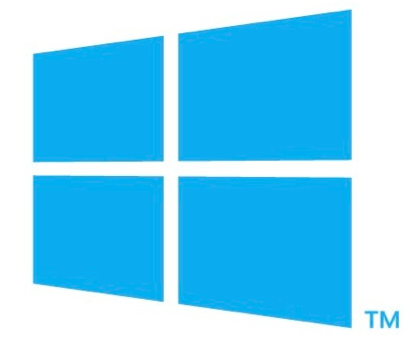
\includegraphics[scale=0.35]{bitmaps/win8logo}
\end{center}

\subsection{Web-Portal (ELMS)}

Wenn du beim Herrn Plass nach dem Zugang zum Web-Portal von Dreamspark Premium \textbf{freundlich} nachfragst, wird er dich nach deiner Uni-E-Mail-Adresse nachfragen, wodurch bestätigt werden kann, dass du bei uns studierst.

In Kürze darauf bekommst du eine E-Mail mit den Logindaten zum Portal. Dort kannst du dann sowie die Distributionen der Softwareprodukte herunterladen, als auch die Lizenzen für dich generieren lassen.

Momentan sind im ELMS \textbf{163 (!)} Produkte verfügbar, darunter Windows 8 Professional, Windows~7 Professional, Visual Studio 2012, Visio 2013, Access 2013 usw.

Dieser Verfahren macht das Erhalten von Lizenzen und Distributionen unkompliziert und nach einmaliger persönlicher Meldung bis zum Ende des Studiums von zu Hause möglich.

\subsection{Manuelle Verwaltung}

RBI verwaltet die Lizenzen zu einigen insbesondere populären Produkten auch manuell. Wenn du \textbf{freundlich} nachfragst, gibt Herr Plass dir einen \textbf{Produktschüssel} für eine entsprechende Lizenz, wenn die Lizenz, \textbf{die du brauchst,} da ist.
% Microsoft darf nur die Liste der E-Mails zwecks Kontrolle, dass Lizenzen nicht verkauft werden, einsehen, also ist die Bemerkung irrelevant.
%Außerdem gibt es da alle Lizenzen aus dem Microsoft DreamSpark Premium Programm (ehemaliges MSDN-AA) so anonym wie möglich (Microsoft darf einmal im Jahr die Daten einsehen aber nicht kopieren oder speichern).

Diese Verwaltungsart ist für die Fälle sinnvoll, wo man aus irgendwelchen Gründen mehrere Lizenzen zu einem populären Softwareprodukt studienbedingt braucht (z.B. zwecks Analyse der gleichzeitigen Ausführung zweier Virtuellen PCs).

Dadurch Wer da aber unbedingt mit den Worten "Gib so viele Lizenzen, wie du hast!" 20 Lizenzen auf einmal haben will, sorgt nur dafür, dass solche Angebote in Zukunft nicht mehr von der Uni bezahlt werden und euch kostenlos zur Verfügung gestellt werden. Also nutzt das Angebot, aber nutzt es nicht aus!

Natürlich reicht die Lizenznummer für die Installation nicht. Du brauchst also noch ein \textbf{Installationsmedium}. Bei der RBI werden nicht Hunderte von CDs und DVDs gelagert. Jeder brennt sich eins selbst (das ist auch völlig legal, wen das interessiert ;)).

Die RBI hat normalerweise ein Distributions-CD zu jedem Programm, das du für ein paar Tage zum Kopieren ausleihen könntest.
Als eine Alternative für die Windows-Betriebsysteme, die sonst mehrmals täglich ausgeliehen wären, kannst du die bereits angefertigten Images\footnote{Digitalisierte Versionen der CDs und der DVDs} aus dem RBI-Netzwerk verwenden:
\begin{wrapfigure}[12]{r}{0.5\textwidth}
     \vspace{12mm}
   \begin{center}
     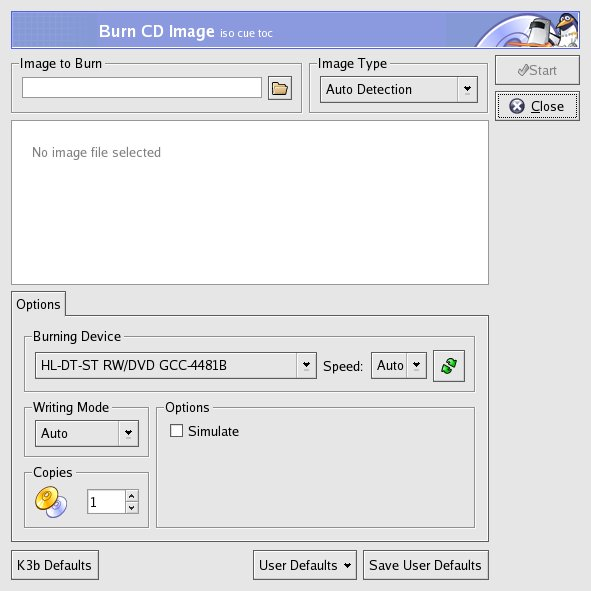
\includegraphics[scale=0.39]{bitmaps/gimp_brennen4}
   \end{center}
\end{wrapfigure}
\begin{enumerate}
\item Hole dir ein [DVD-]Rohling
\item Logge dich an einem der RBI-PCs ein (z.B. in den Fischerräumen)
\item Starte \texttt{k3b} z.B. in der Konsole
\item Gehe im Menü zu\\"Tools"'$\to$"Burn CD Image".

\item Nun muss du dass Image auswählen welches du brennen möchtest:\\
Klicke auf den ''wähle Datei'' Knopf 
\includegraphics[scale=0.5]{bitmaps/gelbe_ordner}, im Bereich ''Image to Burn'' und schau in diesem Ordner nach:

\begin{center}
	\framebox{ \textbf{ \textsf{/opt/rbi/ms\_windows\_iso/} } }
\end{center}
\item Danach wird die Isodatei überprüft. Das wird ein paar Sekunden dauern.

	Sobald dieser Prozess fertig ist, kann man auf den ''Start" Knopf klicken und damit das Brennen starten.

\end{enumerate}

Alternativ kannst du diese Images auf dein USB-Stick kopieren und bequem zu Hause brennen (zum Brennen von Images unter Windows kann man dafür das kostenlose Programm ImgBurn\footnote{\url{http://www.imgburn.com/}} verwenden).

\begin{flushright}Pavel und Jonathan \end{flushright}
